\chapter{Parameter Inference with Bifurcation Diagrams}
\label{chapter:inference}
\begin{music}
    \parindent10mm \instrumentnumber{1} \setstaffs1{1} 
    \generalmeter{\meterfrac44} \generalsignature{2}
    \startextract
            \notes \ql j \ql i \Qqbl ieji \en
        \bar \zw{m*} \bar 
            \notes \ql i \qu h \Qqbu hdih \en
        \bar \zw{l*} 
    \zendextract
\end{music}
\epigraph{\textit{the melody that will draw you into the infinite darkness}}{Nocturne of Shadow --- Ocarina of Time}

\section{Preface}
\subsection{Problem Statement \& Context}

This chapter focuses on the problem of looking for parameter regimes for dynamical systems that result in bifurcations. This has been coined as \emph{inverse bifurcation analysis} \cite{Lu2006InverseSystems}. Formally we are looking for parameters $\theta$ for which the equation \eqref{eq:differential-equations} has at least one fixed point for which bifurcation criteria (see Section \ref{section:bifurcation-analysis}) are satisfied. These bifurcations are to be placed along control condition $p\in\Reals$.

Inverse bifurcation analysis becomes relevant to biomedical researchers in settings where there is a design goal to engineer an organism with a distinct phenotype (as discussed in Chapter \ref{chapter:introduction}).
Such a phenotype can be a the \emph{double exclusive reporter} investigated in the interdisciplinary collaboration in synthetic developmental biology presented in Chapter \ref{chapter:double-exclusive}. This \emph{E. Coli} phenotype exhibits a cusp bifurcation leading to a bistable response with respect to two input signals as shown in Figure \ref{fig:double-exclusive:bistability}. The engineering goal could be a phenotype with a specific cell cycle \cite{Attila2008,Conrad2006BifurcationClock} which involves the positioning of \emph{Hopf bifurcations} that mark the onset of oscillations in protein concentrations from stable equilibria. Finally the design of self-organised patterns such as stripes and spots in mammalian coat patterns could be another engineering goal. According to a long standing mathematical hypotheses \cite{Turing1952} that underpins developmental mechanisms this may involve the search for \emph{Turing bifurcations}.

Before we get carried away and think that with the right tooling we could genetically control the length scale of spots or stripes on cats, we must remind ourselves that \emph{in vivo} gene regulatory networks mostly consist of unknown and experimentally inaccessible parameters. Furthermore, we find that usually there exist multiple equally valid models that describe the observed behaviour, and so turn to \emph{model selection} methods. Even if we had an accurate and unique model to describe an organism, generic tools for \emph{inverse bifurcation analysis} are limited as we've explored in Chapter \ref{chapter:background} and experienced in practice in Chapter \ref{chapter:double-exclusive}. In an attempt to address these limitations, the incorporated publication (sections \ref{inference:abstract} -- \ref{inference:impact}) focuses on the design of systems of ordinary differential equations with \emph{pitchfork} and \emph{saddle-node} bifurcation diagrams. Although the publication focuses on parameter synthesis for a subset of bifurcations, steps towards \emph{Hopf} bifurcations are made (see Appendix \ref{appendix:hopf-measure}), and the approach lays foundations for differentiable optimisation methods that leverage bifurcation theory. A view towards how this approach can be used for the design of \emph{Turing patterns} and model selection is discussed in concluding Chapter \ref{chapter:conclusions}.

\subsection{Contributions}

\textbf{Grisha Szep} prepared the manuscript, designed the cost function, derived mathematical results, wrote and released the Julia package under the supervision of \textbf{Neil Dalchau} and \textbf{Attila Czikasz-Nagy}.

\subsection{An Alternative Approach}
\label{section:field-inference}

In this early days of this thesis, we investigated whether it was possible to transform the time-domain data into state-space. This approach is discussed in this section and can in principle be used with microfluidic fluorescence microscopy data in a \emph{design--learn} workflow (Figure \ref{fig:experimental-design}).

Consider we are given $K$ cell trajectories $\mathcal{D}_1$, $\mathcal{D}_2$ ... $\mathcal{D}_K$, each containing $N$ noisy observations of the state of the cell. Let the cell state be represented by state vector $u(t)\in\Reals^N$ which is hypothesized to obey a set of ordinary differential equations of the form \eqref{eq:differential-equations}. Instead of integrating the equations \eqref{eq:differential-equations} we would find an estimate for the derivative of the trajectories $\hat{f}$.

This is known as the \textit{smoothing} step \cite{Gugushvili2012Smoothing} should be done using unsupervised methods, for example with Gaussian Process Regressors \cite{Seeger2004GaussianLearning.} as shown in in Figure \ref{fig:inferred-cycles}. This requires the inversion of an $K'\times K'$ data matrix where $K':=\sum_k |\mathcal{D}_k|$ is the total number of trajectory data points. This has a computational complexity $K'^3$ which is only tractable with sparse datasets.

Let the region $\partial\mathcal{D}$ be a boundary defined by the Delaunay tessellation of the input data. Let us define the estimate $\hat f$ only within the region $\partial\mathcal{D}$ so that there are no extrapolation artefacts. For the Gaussian Process approach the estimate would be
\begin{equation}
    \hat{f}(u)\sim
        \mathcal{N}(\,\mu(u) ,\Matrix{\Sigma}(u)\,)
    \quad\mathrm{for}\quad u\in\partial\mathcal{D}
\end{equation}
\noindent where at any given state $u$ the field estimate $\hat{f}$ is generated by Gaussian distributions of mean vector $\mu$ and covariance matrix $\Matrix{\Sigma}$. Solving for these requires a choice of matrix-valued kernel function $\Matrix{K}(u,v)$ which encodes our knowledge about the local structure of the field. Sophisticated kernels for learning vector fields exist \cite{Fuselier2017ADecompositions} for decomposing fields in conservative and solenoidal components, which aid in localising fixed points and cycles.

The simplest choice of kernel assumes the components are independent and have a finite correlation length $\gamma$, such as Gaussian radial basis functions. Here $\Matrix{I}$ is the identity matrix and the hyperparameter $\gamma$ has to be optimised.
\begin{equation}
    \Matrix{K}(\Vector{u},\Vector{v}) = \Matrix{I}\,\mathbb{e}^{-\gamma|\Vector{u}-\Vector{v}|^2}
\end{equation}

The second step is called \textit{matching} where the estimated field $\hat{f}$ is used as an optimisation target against some parametrised function $\rates$ with unknown parameters $\theta$.

In our setting we would like to match the geometry of the field but not its magnitude; in this sense we are focusing on the qualitative aspects of the dynamics of a set of differential equations, rather than the quantitative dynamics or kinetics. This could be achieved with the following objective function
\begin{equation}
    \mathcal{L}(\theta|\mathcal{D}) := \e^{-\frac{\hat{f}\cdot\rates}
    {|\hat{f}||\rates|}}
	\label{eq:geometric-cost}
\end{equation}
\noindent where the cost is minimal when the data derivative $\hat{f}$ and the parametrised model $\rates$ point in the same direction and maximal when they point in opposing directions.

\begin{Figure}
    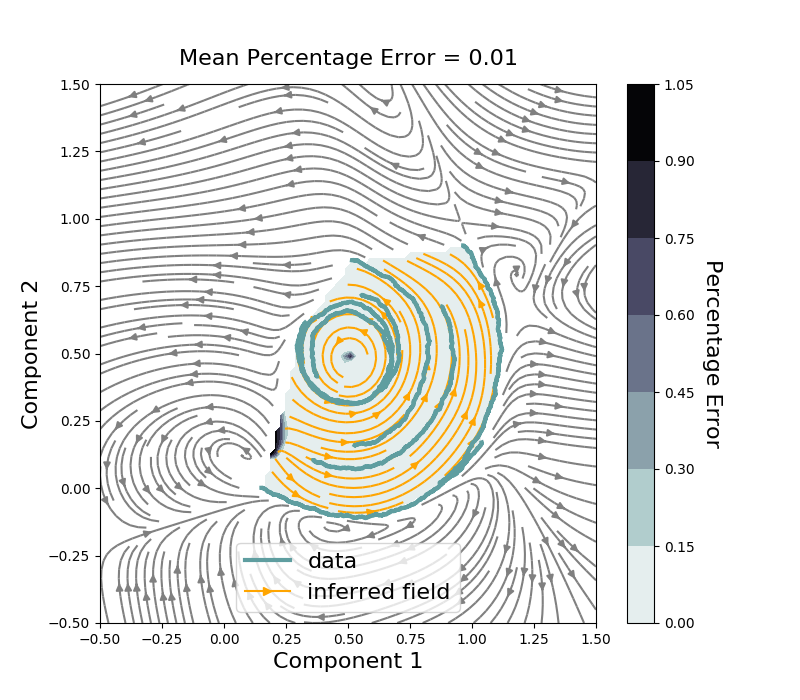
\includegraphics[width=125mm]{figures/cycle-2.png}
    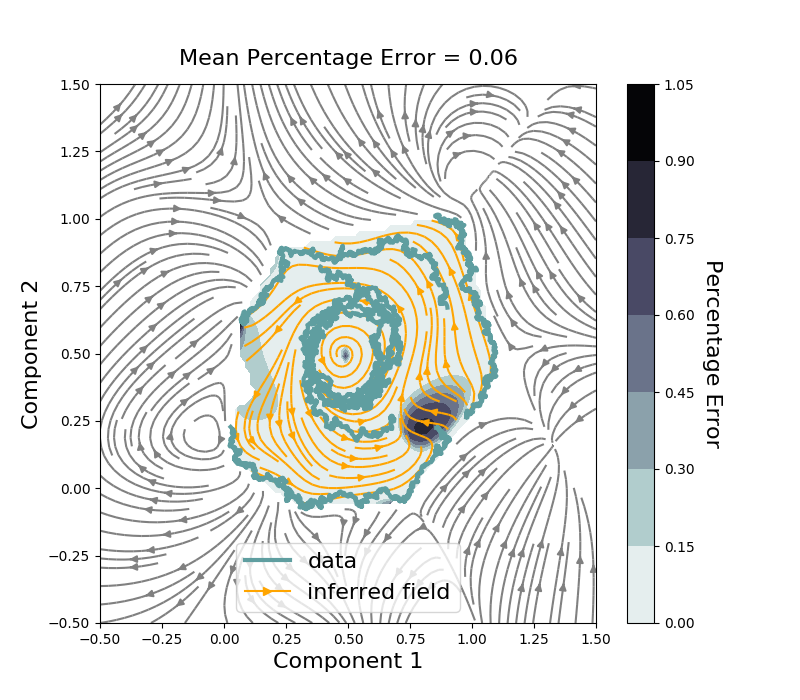
\includegraphics[width=125mm]{figures/cycle-1.png}
    \caption{Gaussian process regressors estimating derivative of the trajectories $\hat{f}$ from example trajectory datasets $\mathcal{D}_1$ ... $\mathcal{D}_K$ with varying signal to noise ratios. Interpolation error $E$ is shown as a heatmap; extrapolation fails}
    \label{fig:inferred-cycles}
\end{Figure}

The accuracy of the cell trajectories is limited by cell segmentation and tracking algorithms. Initial investigations into this approach also suggested that trajectories need to be of sufficient temporal resolution and sampled from a wide variety of initial conditions. Such data is not widely available and ultimately we decided to focus on a method that could be used with a well-known workhorse in biomedical research: flow cytometry.

Although we are getting close to focusing on qualitative features of a model, this objective function \eqref{eq:geometric-cost} is still sensitive to the locations and shapes of fixed point and limit cycles. What if we cared about even higher-level features such as the number of fixed points? Or perhaps whether a system oscillates or not? This is where the language of bifurcation theory described in Chapter \ref{chapter:background} is optimally suited for this task.

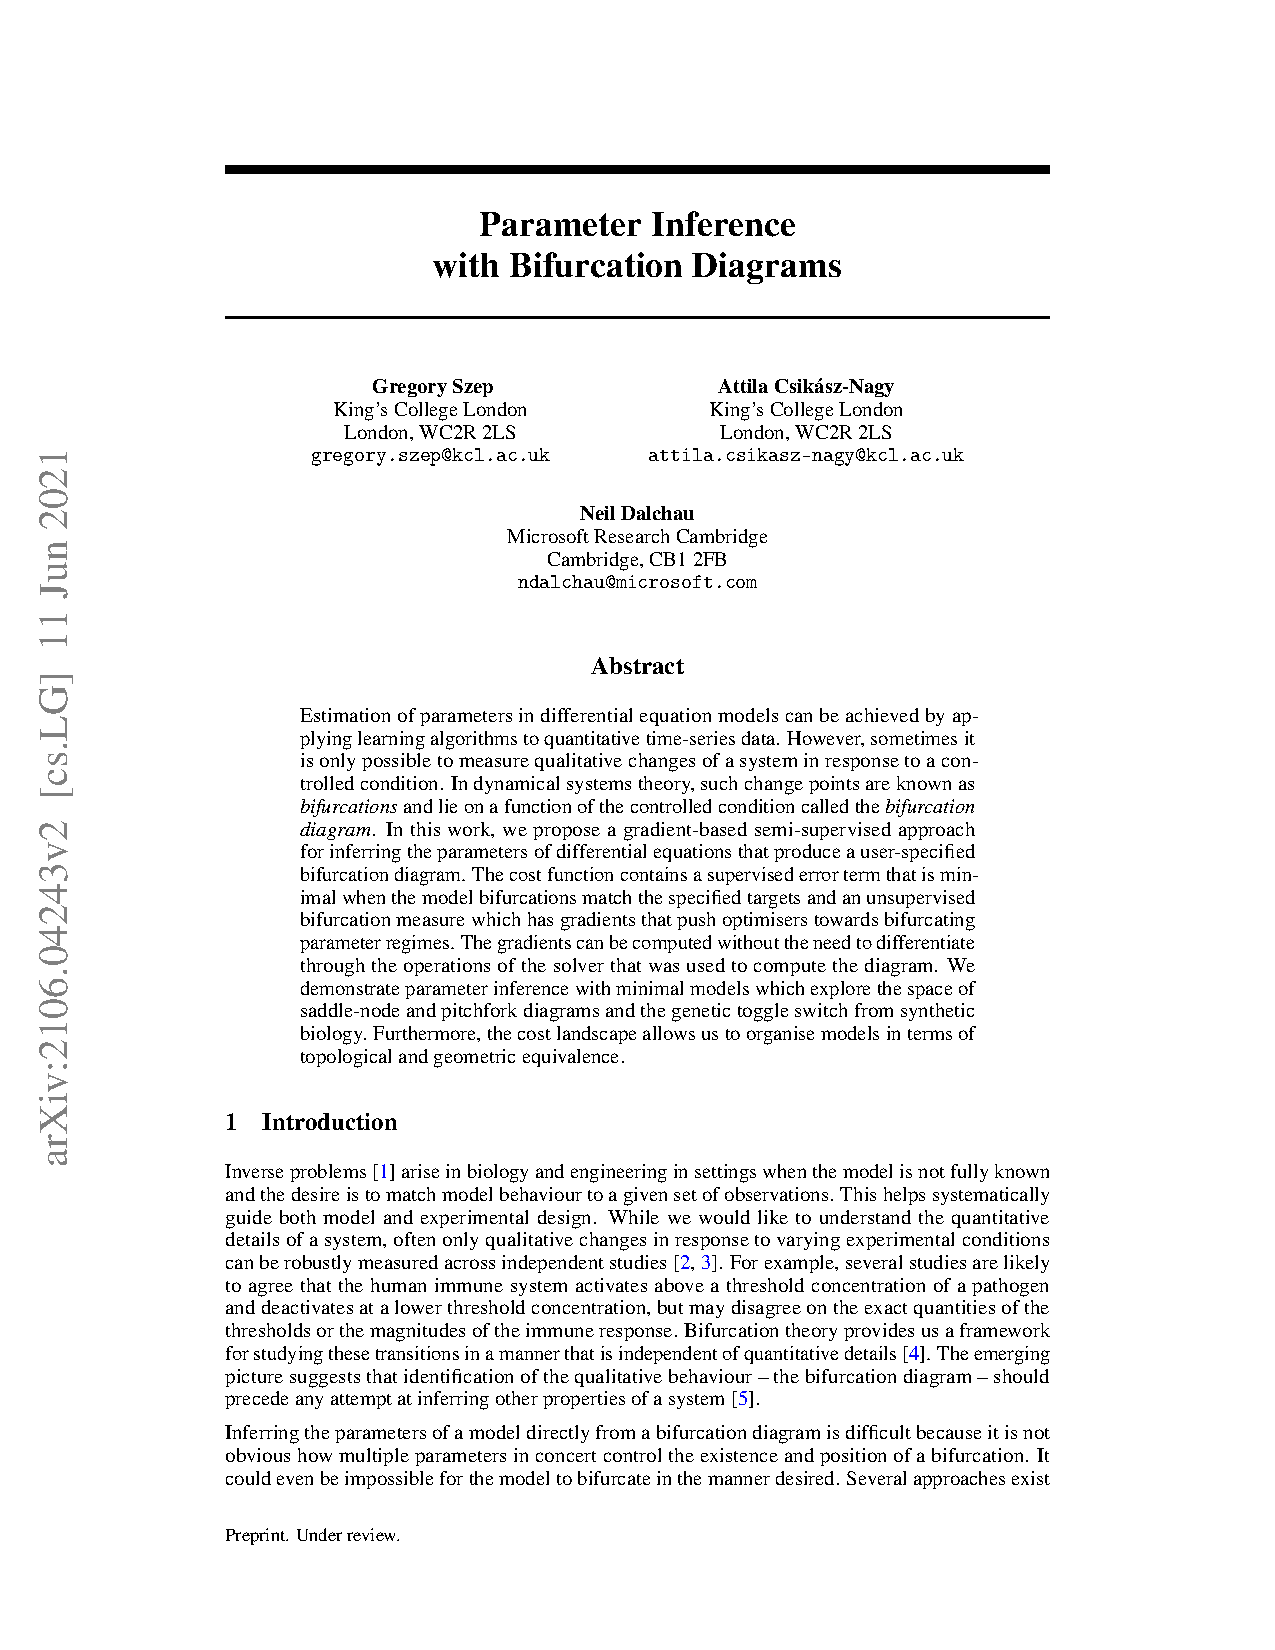
\includepdf[pages=1-11, offset=75 -95, scale=0.85, frame,
        clip,trim=31mm 21mm 31mm 21mm,
        pagecommand={}, addtotoc={
        1,section,1,Abstract,inference:abstract,
        1,section,1,Introduction,inference:introduction,
        2,subsection,2,Preliminaries,inference:preliminaries,
        4,section,1,Proposed Method,inference:method,
        4,subsection,2,Semi-supervised Cost Function,inference:cost,
        5,subsection,2,Differentiating the semi-supervised cost function,inference:derivatives,
        6,section,1,Experiments \& Results,inference:results,
        6,subsection,2,Minimal Models,inference:minimal,
        6,subsection,2,Genetic Toggle Switch,inference:genetic,
        7,subsection,2,Complexity,inference:complexity,
        9,section,1,Conclusion \& Broader Impact,inference:impact,
        10,section,1,References,inference:references},
    addtolist={
        3, figure, {\textit{Fig. 1}\quad Illustration of bifurcation diagrams for minimal models of bifurcations. A. Saddle-node bifurcations arise for $\rates(u,p) = p + \theta_{1}u+\theta_{2}u^3$ when $\theta = (\frac{5}{2},-1)$. B. Pitchfork bifurcations arise for $\rates(u,p) = \theta_{1} + p u+\theta_{2}u^3$ when $\theta=(\frac{1}{2},-1)$. Targets are illustrated by light yellow vertical lines. Bifurcation curves are shown as solid blue and red lines, with lighter shades indicating the determinant crossing zero at locations $\predictions(\theta)$ giving rise to unstable solutions.}, fig:inference:minimal-models,
        4, figure, {\textit{Fig. 2}\quad Bifurcation measure $\measure(s)$ and determinant $\Det$ along the arclength $s$ of two different bifurcation curves demonstrating how maximising the measure along the curve maintains the existing bifurcation marked by a circle, while encouraging new bifurcations marked by stars.}, fig:inference:measure,
        6, figure, {\textit{Fig. 3}\quad Saddle-node $\rates(u,p) = p + \theta_{1}u+\theta_{2}u^3$ and pitchfork $\rates(u,p) = \theta_{1} + u p +\theta_{2}u^3$ optimised with respect to $\theta$ so that predicted bifurcations $\predictions(\theta)$ match targets $\targets$ in control condition $p$. The right panel shows bifurcations diagrams for the three optimal $\theta^*$ marked by stars on the left panel. The optimisation trajectories in white follow the gradient of the cost, approaching the black lines of global minima in the left panel}, fig:inference:minimal-models:results,
        7, figure, {\textit{Fig. 4}\quad Bifurcation inference for the two-state model (11). A. Optimal parameter estimates $\theta^*$ for the targets $\targets=\{4,5\}$ reveal two clusters of qualitatively different regimes: mutual activation ($a_1 < 1$; cluster 1) and mutual inhibition ($a_1 > 1$; cluster 2). B. Example bifurcation diagrams indicate positively and negatively correlated dependencies between the two model states, as a function of the control condition.}, fig:inference:two-state-optima,
        8, figure, {\textit{Fig. 5}\quad A. Execution time (time to calculate cost gradient) with respect to states $N$. B. Convergence times (the time it takes to find and match a bifurcation to within 1\% of a specified target) with respect to the number of parameters $M$, comparing against a gradient-free approach: Nelder-Mead. Calculations were performed on an Intel Core i7-6700HQ CPU @ 2.60GHz x 8 without GPU acceleration.}, fig:scaling
}]{publications/bifurcation-inference.pdf}

\section{Afterword}
\begin{itemize}
    \item extension to cusp bifurcation
    \item extension to spatial system and turing
    \item designing limit cycles
\end{itemize}